\clearpage
\section{Analysis and Discussion}


\subsection{Task 1}

在訓練 A2C 的時候,我發現我的模型會請向 +2 或是 -2 的力矩,從影片中也可以看到,這個 Agent 在上方保持穩定的策略,也是快速的在力矩的方向上交換。

\begin{figure}[h]
    \centering
    \begin{subfigure}[b]{0.8\textwidth}
        \centering
        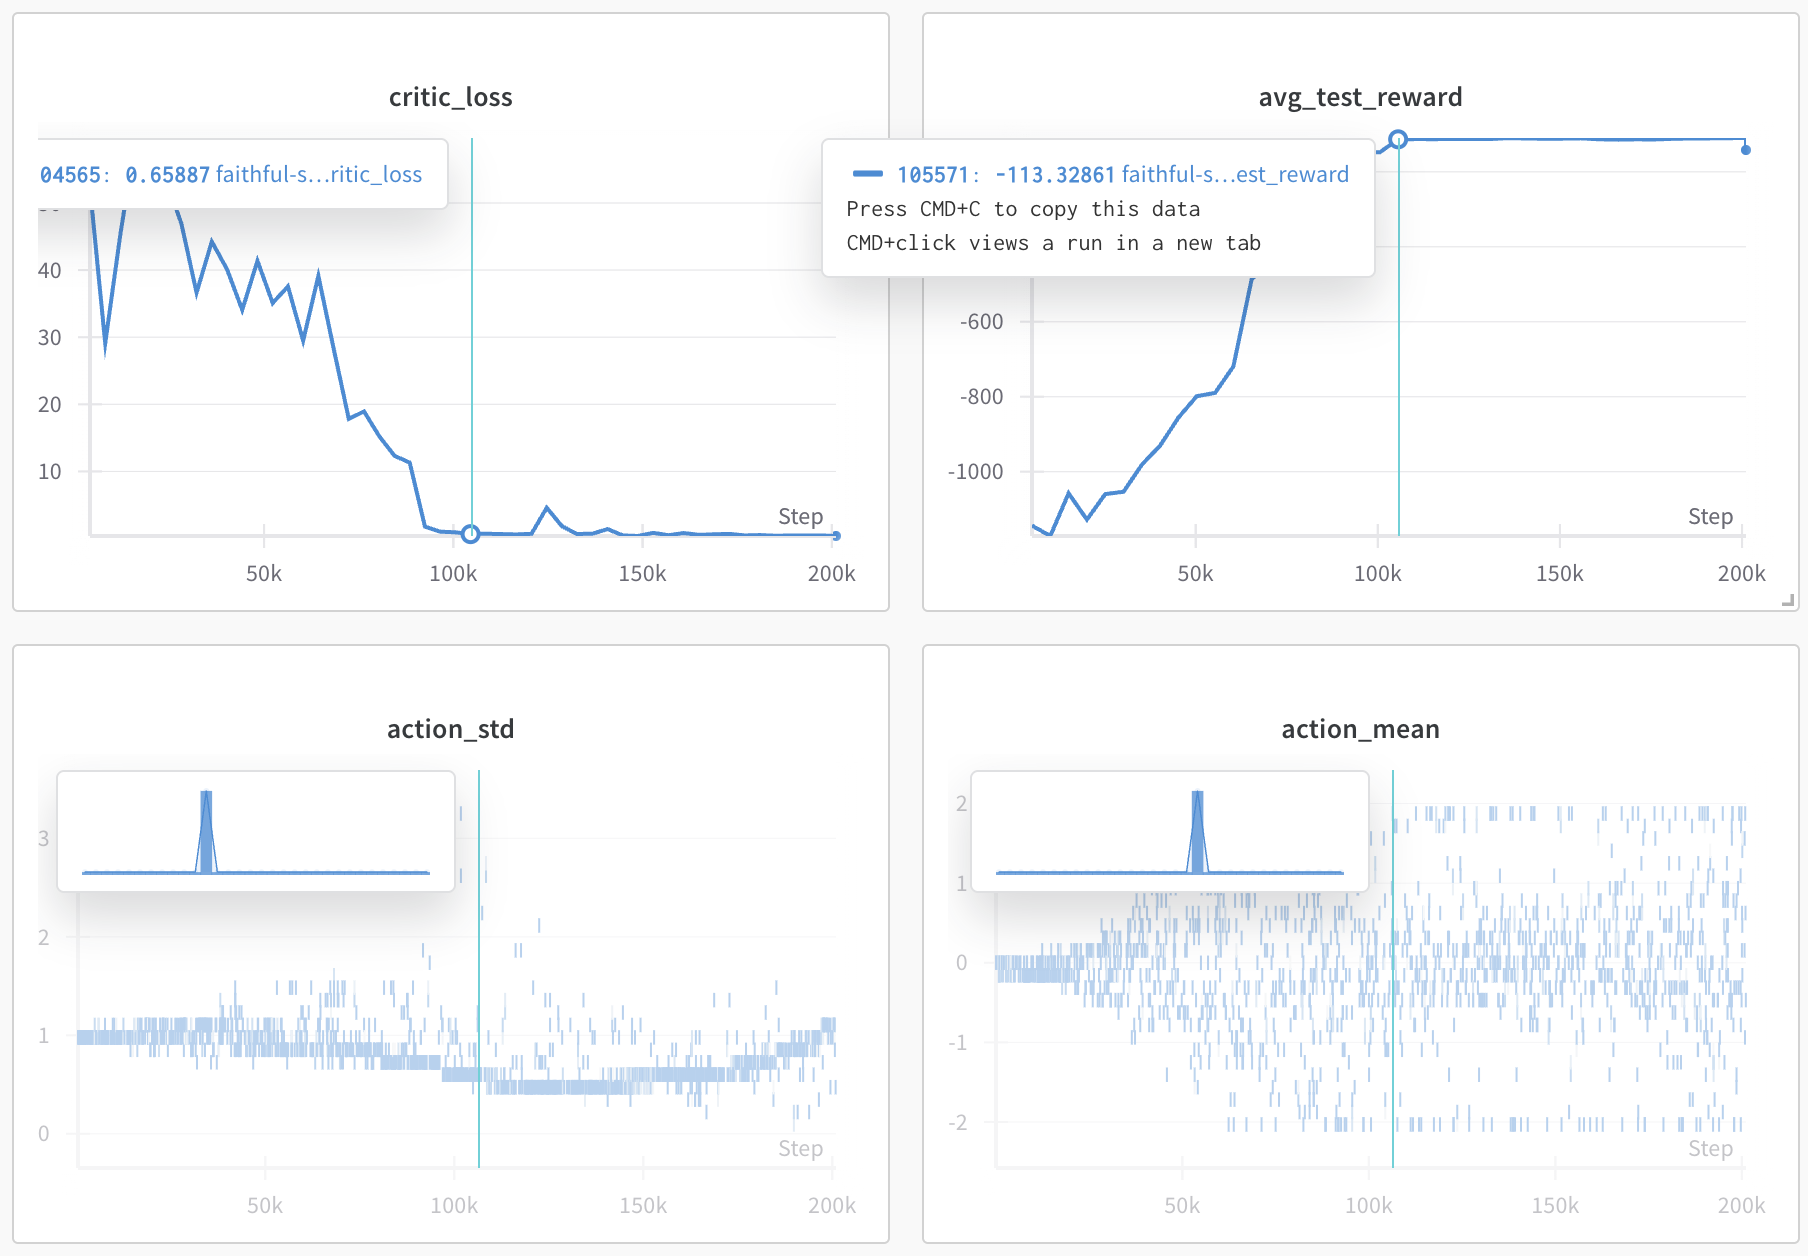
\includegraphics[width=\textwidth]{figures/A2C_action_dist.png}
        \caption{A2C 動作分布圖}
        \label{fig:a2c_action_dist}
    \end{subfigure}
    \vspace{0.5cm}
    \begin{subfigure}[b]{0.8\textwidth}
        \centering
        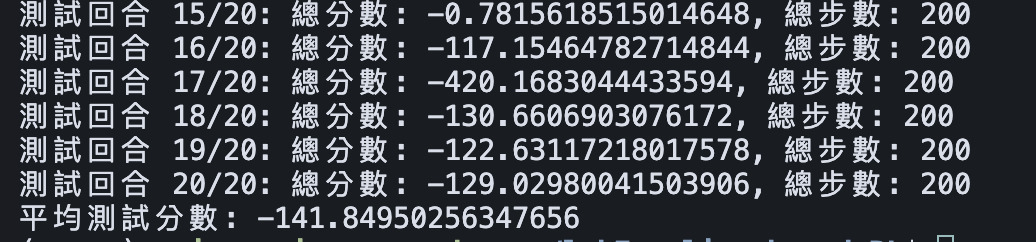
\includegraphics[width=\textwidth]{figures/task1_test_value.png}
        \caption{Task 1 測試值}
        \label{fig:task1_test_value}
    \end{subfigure}
    \caption{Task 1 的動作分布與測試值}
    \label{fig:task1_combined}
\end{figure}

可見模型在 A2C 的訓練方法中,還沒辦法學習到在上方使用小力矩的穩定策略。

\begin{figure}[h]
    \centering
    \begin{subfigure}[b]{0.48\textwidth}
        \centering
        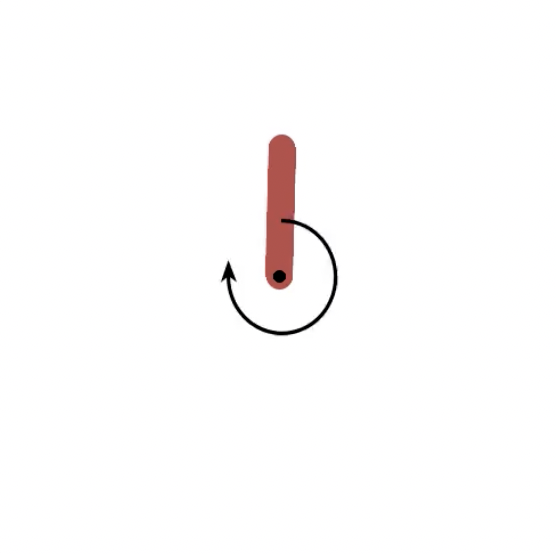
\includegraphics[width=\textwidth]{figures/task1_frame1.png}
        \caption{Frame 1}
        \label{fig:task1_frame1}
    \end{subfigure}
    \hfill
    \begin{subfigure}[b]{0.48\textwidth}
        \centering
        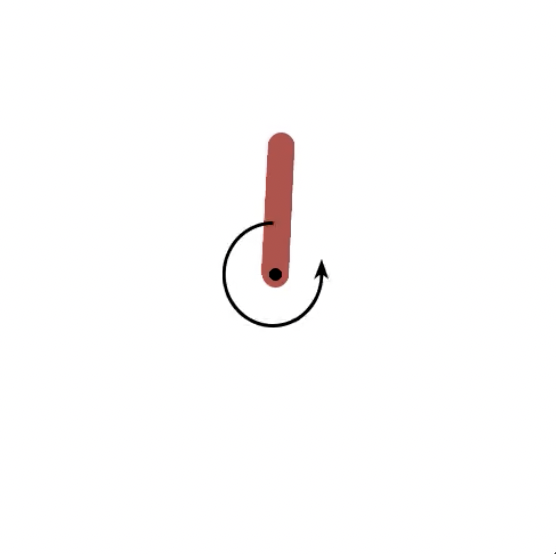
\includegraphics[width=\textwidth]{figures/task1_frame2.png}
        \caption{Frame 2}
        \label{fig:task1_frame2}
    \end{subfigure}
    \caption{Task 1 的策略示意圖}
    \label{fig:task1_frames}
\end{figure}


\clearpage
\subsection{Task 2}


使用 PPO 訓練的 agent 在 task 2 中,就比較容易學習到在上方使用小力矩的穩定策略,這裡比較有趣的是,小的 batch size 顯著的學習比較快,如同 exp 11 與 12,但是有個問題就是,當達到最優策略之後, reward 會快速坍塌,回到 -1000 左右的水準,至今還是很迷茫。

\begin{figure}[h]
    \centering
    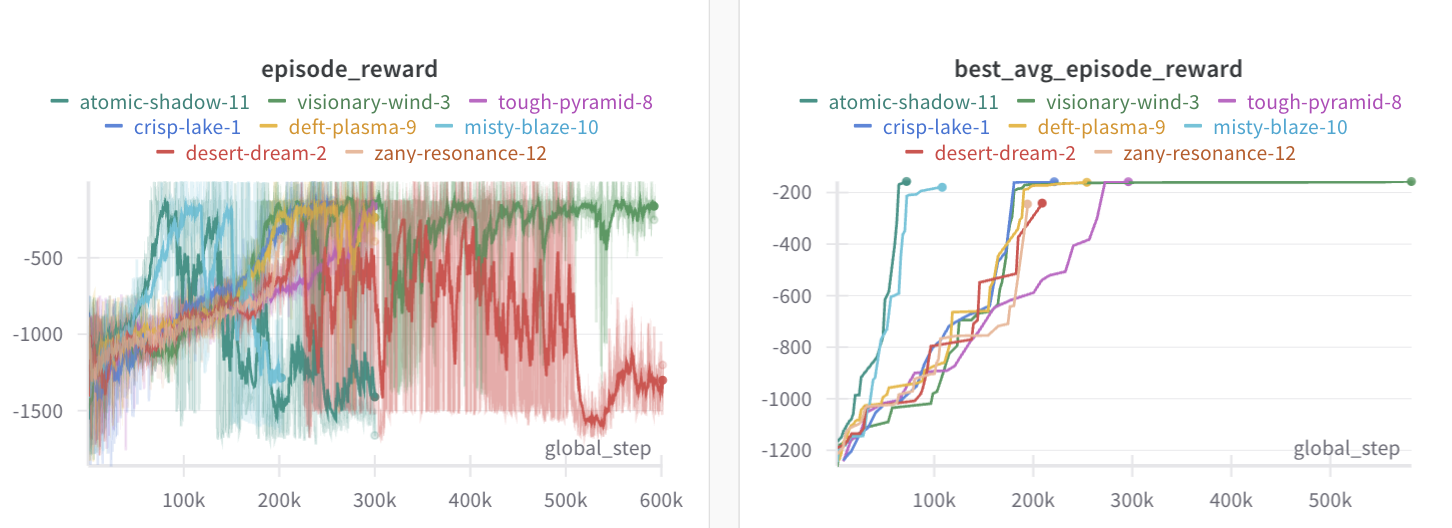
\includegraphics[width=\textwidth]{figures/task2_reward.png}
    \caption{Task 2 的獎勵值變化}
    \label{fig:task2_reward}
\end{figure}

\begin{figure}[h]
    \centering
    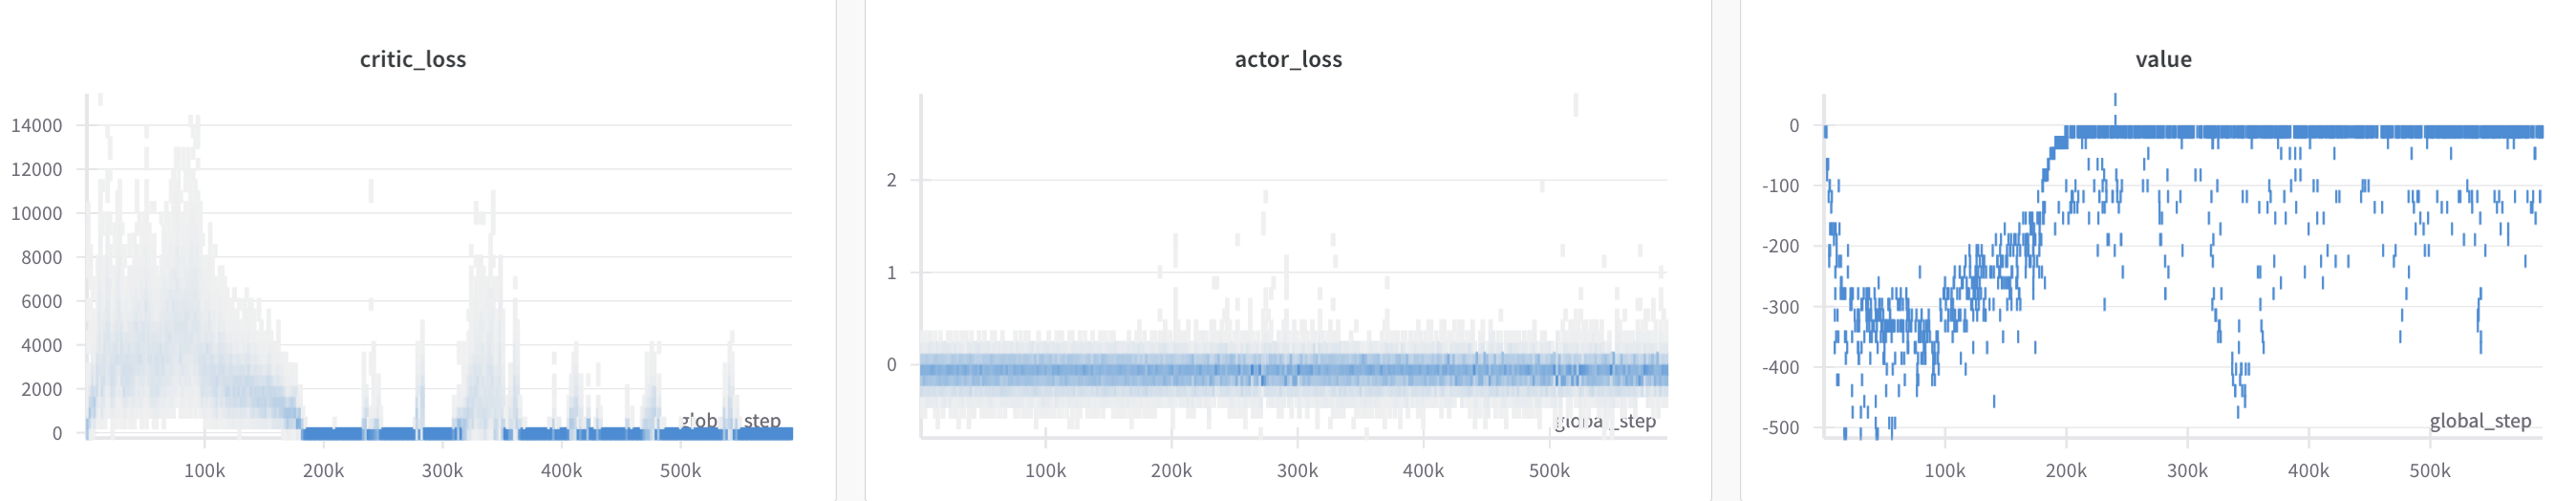
\includegraphics[width=\textwidth]{figures/task2_loss.png}
    \caption{Task 2 的損失值變化}
    \label{fig:task2_loss}
\end{figure}

\clearpage
\subsection{Task 3}

\begin{figure}[h]
    \centering
    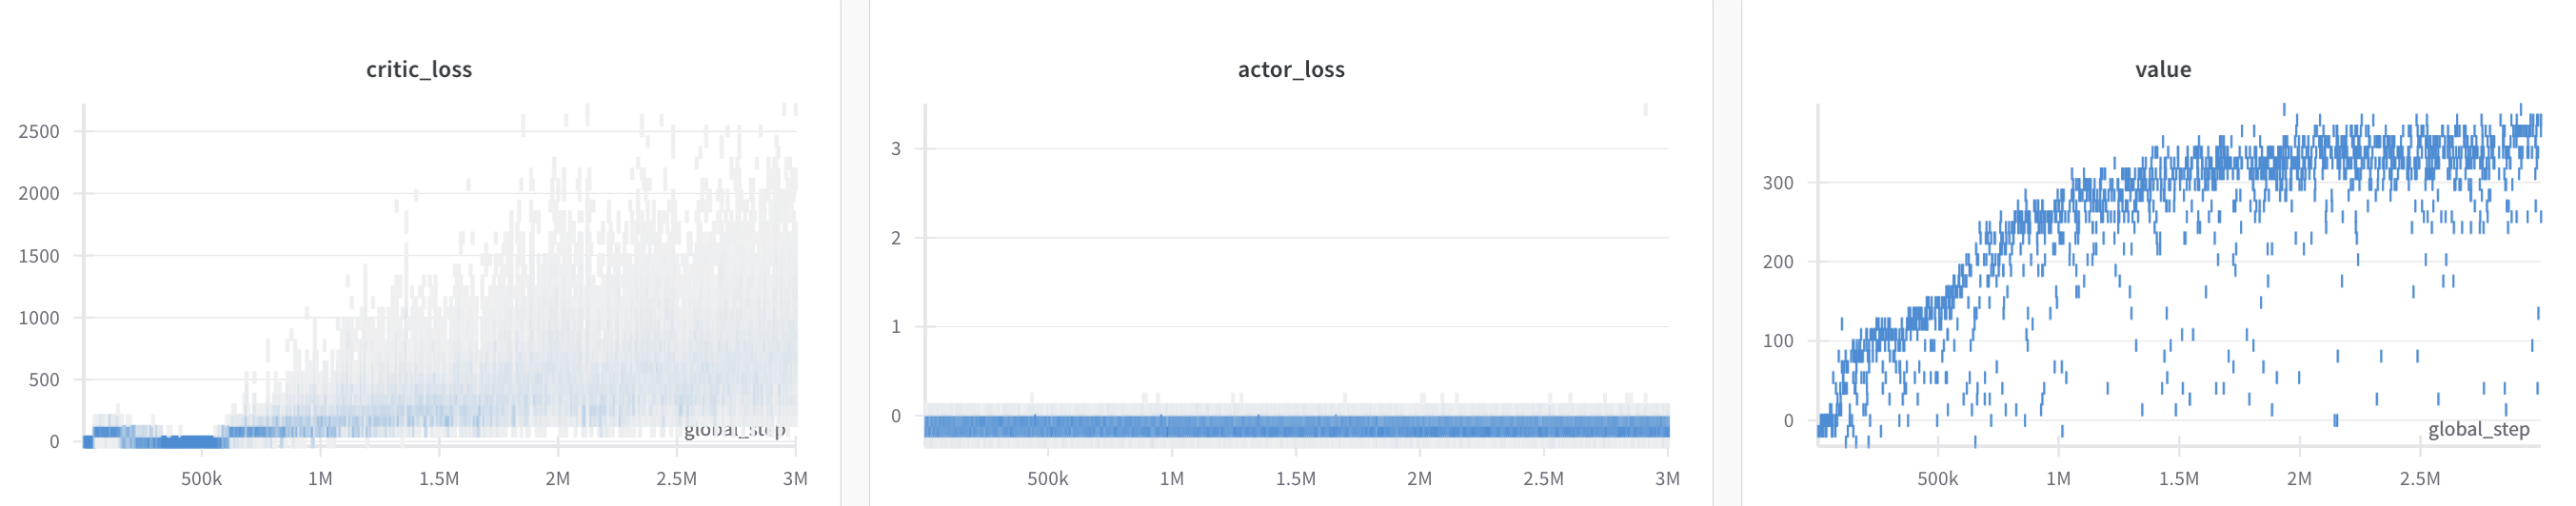
\includegraphics[width=\textwidth]{figures/task3_loss.png}
    \caption{Task 3 的損失值變化}
    \label{fig:task3_loss}
\end{figure}

我覺得在 RL 當中, loss 的數值似乎不太能夠說明是否學習到最佳策略,因為隨著模型越來越厲害,他會遇到越來越多困難的 case,所以 value 會不易預估,所以 loss 會開始發散,所以我覺得在 RL 中,觀察學習是否收斂最好的方法是看 critic Network 的輸出值,如果輸出值能夠穩定,就代表模型學習到最佳策略,因為模型已經能正確判斷任何他遇到的 state 的未來可能收益了。

\begin{figure}[h]
    \centering
    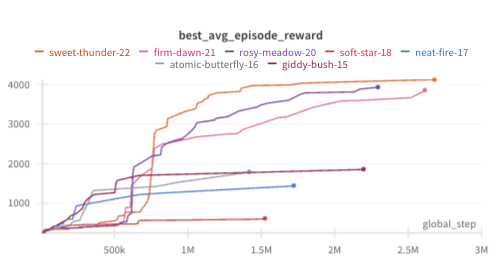
\includegraphics[width=\textwidth]{figures/The importance of exploration.png}
    \caption{探索的重要性與 average reward 示意圖}
    \label{fig:exploration_importance_and_value}
\end{figure}

\clearpage
\subsection{Empirical study: The importance of exploration}

由於我在train 的時候, test average 只使用 5 次平均,並不是作業要求的 20 次,所以之後我在得到最大的 reward 時,我有在使用 20 次平均的 test reward 來證明在 20 次不同 case 都可以得到超過 4000 分。


\begin{figure}[h]
    \centering
    \begin{subfigure}[b]{0.48\textwidth}
        \centering
        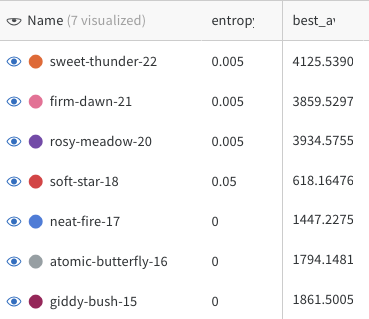
\includegraphics[width=\textwidth]{figures/The importance of exploration value.png}
        \caption{探索值與平均獎勵的關係}
        \label{fig:exploration_value}
    \end{subfigure}
    \hfill
    \begin{subfigure}[b]{0.48\textwidth}
        \centering
        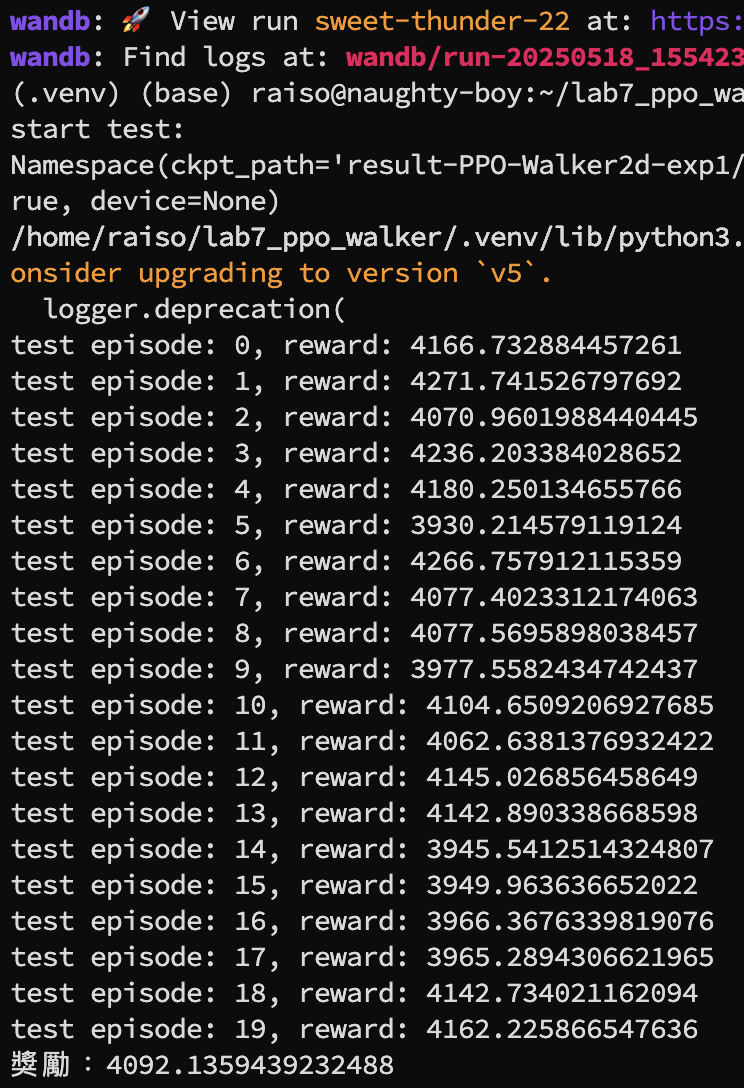
\includegraphics[width=\textwidth]{figures/Top_walk2d_test_result.png}
        \caption{最佳 Walker2d 測試結果}
        \label{fig:top_walk2d_test}
    \end{subfigure}
    \caption{探索值與模型表現的關係}
    \label{fig:exploration_and_performance}
\end{figure}



令我訝異的是,model 學到,先使用後腳跟往後瞪,快速地讓身體前傾至接近 45 度角,然後利用重力,協助 agent 快快往前跑,這真是讓我驚呆了!

\begin{figure}[h]
    \centering
    \begin{subfigure}[b]{0.24\textwidth}
        \centering
        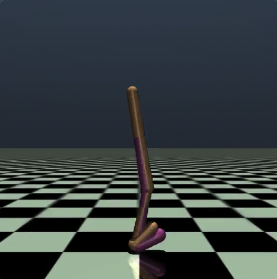
\includegraphics[width=\textwidth]{figures/walk2d-1.png}
        \caption{Step 1}
        \label{fig:walk2d_1}
    \end{subfigure}
    \hfill
    \begin{subfigure}[b]{0.24\textwidth}
        \centering
        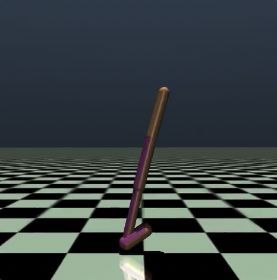
\includegraphics[width=\textwidth]{figures/walk2d-2.png}
        \caption{Step 2}
        \label{fig:walk2d_2}
    \end{subfigure}
    \hfill
    \begin{subfigure}[b]{0.24\textwidth}
        \centering
        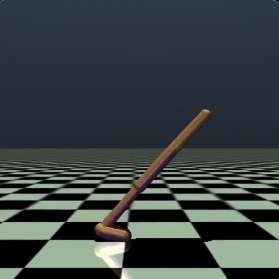
\includegraphics[width=\textwidth]{figures/walk2d-3.png}
        \caption{Step 3}
        \label{fig:walk2d_3}
    \end{subfigure}
    \hfill
    \begin{subfigure}[b]{0.24\textwidth}
        \centering
        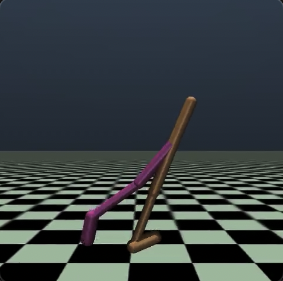
\includegraphics[width=\textwidth]{figures/walk2d-4.png}
        \caption{Step 4}
        \label{fig:walk2d_4}
    \end{subfigure}
    \caption{Walker2d 動作分解圖}
    \label{fig:walk2d_steps}
\end{figure}

\clearpage
\subsection{Additional training strategy: Bayesian Optimization}

在前幾次的作業當中,我意識到了超參數調整的痛苦,所以這次我使用 Wandb 的 Sweep 功能來協助我調整超參數,再加上 Performance 訓練過程其實非常快速,如果需要一直人為設定超參數的話,會導致計算資源的閒置,下圖是我使用 Sweep 的結果:

\begin{figure}[h]
    \centering
    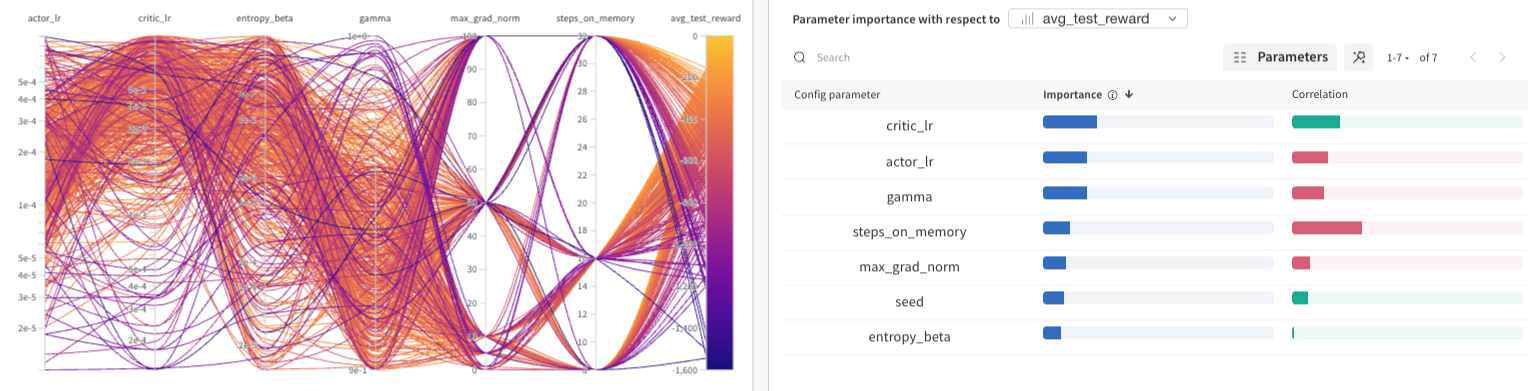
\includegraphics[width=0.8\textwidth]{figures/Sweep Case.png}
    \caption{Wandb Sweep 超參數調整結果}
    \label{fig:sweep_case}
\end{figure}

我使用 Sweep 把超參數當作輸入,使用 Bayesian 的方式,以 average best reward 當作優化目標,讓模型執行 500 次超參數嘗試,這裡我們可以看到大量的實驗累積在 高 critic learning rate 以及 actor learning rate,以及比較多的線累積在 0.9~0.96 的 gamma,這正告訴我們 這裡可以大膽地調高 learning rate,以及 gamma 的值模型其實夠用了,不用設定到 0.99 之類的高數值,另外還有一個小細節,就是 leanring rate 中, critic 其實比 actor 還要更集中在數值大的區域,也就是其實在訓練 PPO 的過程中,模型要先學會 value network 的估計,才會開始學習 policy network 的估計,這也告訴我們,在設定超參數的時候,這也給了我 Walker2d task 訓練時,超參數的啟發,讓我可以在 1M env step 以內就衝上 3000 分。